\section{Harun Ar - Rasyid(1174027)}
\subsection{PYSHP Writer}
\begin{enumerate}
	\item Buatlah Script Python dan jelaskan berbaris
	\lstinputlisting[firstline=2, lastline=11]{src/1174027/2/praktikum.py}
	\begin{itemize}
		\item Untuk baris pertama berfungsi untuk memanggil library PYSHP atau shapefile
		\item Untuk baris kedua berfungsi untuk menggunakan atribute Writer yang digunakan untuk membuat file shp,shx, dan dbf. Dengan parameter nama outputnya.
		\item Untuk baris ketiga dan keempat digunakan untuk membuat field yang akan disimpan pada database, dan tipe data yang digunakannya.
		\item Untuk baris kelima dan keenam digunakan untuk menginputkan data,sesuai dengan jumlah fieldnya.
		\item Untuk baris ketujuh dan kedelapan digunakan untuk menginputkan koordinat(x,y) ,dengan menggunakan point atribute untuk menghasilkan pola titik. \hfill\break
		saat menginputkan data, data dengan jumlah koordinat harus sama, karena berkorespondensi 1 - 1.
		\item Untuk Baris ke Sembilan digunakan untuk mengakhiri proses pembuatan PYSHP.
	\end{itemize}
	\hfill\break
	\begin{figure}[H]
		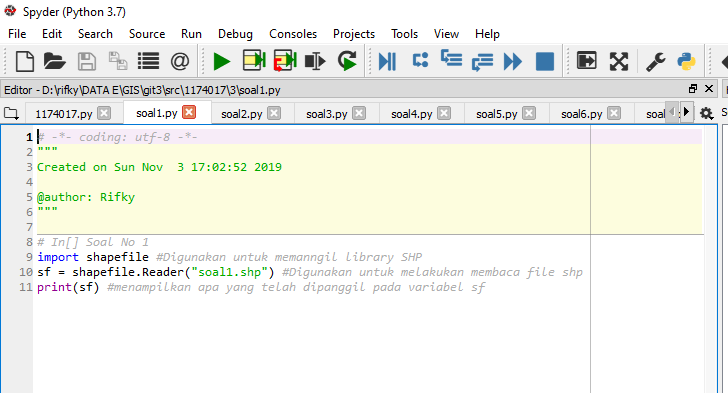
\includegraphics[width=4cm]{figures/1174027/2/soal1.png}
		\centering
		\caption{Hasil SHP Soal 1}
	\end{figure}

	\item Buatlah Script Python dan jelaskan berbaris
	\lstinputlisting[firstline=13, lastline=22]{src/1174027/2/praktikum.py}
	\begin{itemize}
		\item Untuk baris pertama berfungsi untuk memanggil library PYSHP atau shapefile
		\item Untuk baris kedua berfungsi untuk menggunakan atribute Writer yang digunakan untuk membuat file shp,shx, dan dbf. \hfill\break Dengan parameter nama outputnya dan shapeTypenya(shapeType bisa menggunakan angka / namanya).
		\item Untuk baris ketiga dan keempat digunakan untuk membuat field yang akan disimpan pada database, dan tipe data yang digunakannya.
		\item Untuk baris kelima dan keenam digunakan untuk menginputkan data,sesuai dengan jumlah fieldnya.
		\item Untuk baris ketujuh dan kedelapan digunakan untuk menginputkan koordinat(x,y),dengan menggunakan point atribute untuk menghasilkan pola titik. \hfill\break
		saat menginputkan data, data dengan jumlah koordinat harus sama, karena berkorespondensi 1 - 1.
		\item Untuk Baris ke Sembilan digunakan untuk mengakhiri proses pembuatan PYSHP.
	\end{itemize}
	\hfill\break
	\begin{figure}[H]
		
\includegraphics[width=4cm]{figures/1174027/2/soal2.png}
		\centering
		\caption{Hasil SHP Soal 2}
	\end{figure}

	\item Buatlah Script Python dan jelaskan berbaris
	\lstinputlisting[firstline=25, lastline=36]{src/1174027/2/praktikum.py}
	\begin{itemize}
		\item Untuk baris pertama berfungsi untuk memanggil library PYSHP atau shapefile
		\item Untuk baris kedua berfungsi untuk menggunakan atribute Writer yang digunakan untuk membuat file shp,shx, dan dbf. \hfill\break Dengan parameter nama outputnya dan shapeTypenya(shapeType bisa menggunakan angka / namanya).
		\item untuk baris ketiga hingga kelima digunakan untuk menentukan jenis shapeTypenya.
		\item Untuk baris keenam dan ketujuh digunakan untuk membuat field yang akan disimpan pada database, dan tipe data yang digunakannya.
		\item Untuk baris kedelapan dan kesembilan digunakan untuk menginputkan data,sesuai dengan jumlah fieldnya.
		\item Untuk baris kesepuluh dan kesebelas digunakan untuk menginputkan koordinat(x,y),dengan menggunakan point atribute untuk menghasilkan pola titik. \hfill\break
		saat menginputkan data, data dengan jumlah koordinat harus sama, karena berkorespondensi 1 - 1.
		\item Untuk Baris keduabelas digunakan untuk mengakhiri proses pembuatan PYSHP.
	\end{itemize}
	\hfill\break
	\begin{figure}[H]
		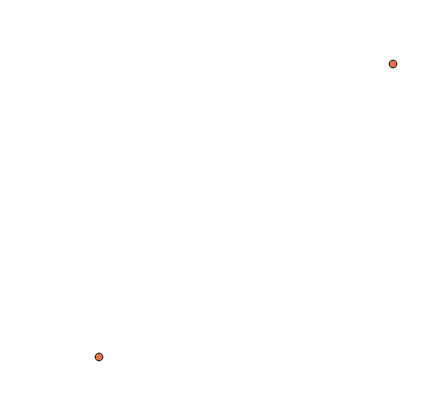
\includegraphics[width=4cm]{figures/1174027/2/soal3.png}
		\centering
		\caption{Hasil SHP Soal 3}
	\end{figure}

	\item Buatlah Script Python dan jelaskan berbaris
	\lstinputlisting[firstline=40, lastline=49]{src/1174027/2/praktikum.py}
	\begin{itemize}
		\item Untuk baris pertama berfungsi untuk memanggil library PYSHP atau shapefile
		\item Untuk baris kedua berfungsi untuk menggunakan atribute Writer yang digunakan untuk membuat file shp,shx, dan dbf. \hfill\break Dengan parameter nama outputnya dan shapeTypenya(shapeType bisa menggunakan angka / namanya).
		\item Untuk baris ketiga dan keempat digunakan untuk membuat field yang akan disimpan pada database, dan tipe data yang digunakannya.
		\item Untuk baris kelima dan keenam digunakan untuk menginputkan data,sesuai dengan jumlah fieldnya.
		\item Untuk baris ketujuh dan kedelapan digunakan untuk menginputkan koordinat(x,y),dengan menggunakan point atribute untuk menghasilkan pola titik. \hfill\break
		saat menginputkan data, data dengan jumlah koordinat harus sama, karena berkorespondensi 1 - 1.
		\item Untuk Baris ke Sembilan digunakan untuk mengakhiri proses pembuatan PYSHP.
	\end{itemize}
	\hfill\break
	\begin{figure}[H]
		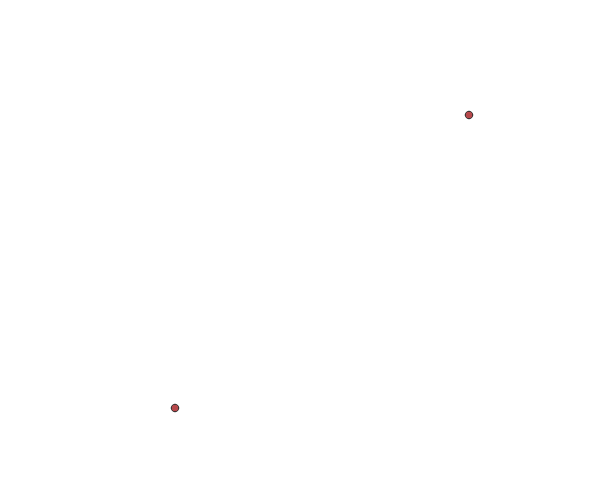
\includegraphics[width=4cm]{figures/1174027/2/soal4.png}
		\centering
		\caption{Hasil SHP Soal 4}
	\end{figure}

	\item Buatlah Script Python dan jelaskan berbaris
	\lstinputlisting[firstline=53, lastline=60]{src/1174027/2/praktikum.py}
	\begin{itemize}
		\item Untuk baris pertama berfungsi untuk memanggil library PYSHP atau shapefile
		\item Untuk baris kedua berfungsi untuk menggunakan atribute Writer yang digunakan untuk membuat file shp,shx, dan dbf. \hfill\break Dengan parameter nama outputnya dan shapeTypenya(shapeType bisa menggunakan angka / namanya).
		\item Untuk baris ketiga digunakan untuk menentukan jenis shapeTypenya.
		\item Untuk baris keempat dan kelima digunakan untuk membuat field yang akan disimpan pada database, dan tipe data yang digunakannya.
		\item Untuk baris keenam digunakan untuk menginputkan data,sesuai dengan jumlah fieldnya.
		\item Untuk baris ketujuh digunakan untuk menginputkan koordinat(x,y), dengan menggunakan line atribute untuk menghasilkan pola line. \hfill\break
		saat menginputkan data, data dengan jumlah koordinat harus sama, karena berkorespondensi 1 - 1.
		\item Untuk Baris kedelapan digunakan untuk mengakhiri proses pembuatan PYSHP.
	\end{itemize}
	\hfill\break
	\begin{figure}[H]
		
\includegraphics[width=4cm]{figures/1174027/2/soal5.png}
		\centering
		\caption{Hasil SHP Soal 5}
	\end{figure}

	\item Buatlah Script Python dan jelaskan berbaris
	\lstinputlisting[firstline=63, lastline=70]{src/1174027/2/praktikum.py}
	\begin{itemize}
		\item Untuk baris pertama berfungsi untuk memanggil library PYSHP atau shapefile
		\item Untuk baris kedua berfungsi untuk menggunakan atribute Writer yang digunakan untuk membuat file shp,shx, dan dbf. \hfill\break Dengan parameter nama outputnya dan shapeTypenya(shapeType bisa menggunakan angka / namanya).
		\item Untuk baris ketiga digunakan untuk menentukan jenis shapeTypenya.
		\item Untuk baris keempat dan kelima digunakan untuk membuat field yang akan disimpan pada database, dan tipe data yang digunakannya.
		\item Untuk baris keenam digunakan untuk menginputkan data,sesuai dengan jumlah fieldnya.
		\item Untuk baris ketujuh digunakan untuk menginputkan koordinat(x,y), dengan menggunakan line atribute untuk menghasilkan pola line. \hfill\break
		saat menginputkan data, data dengan jumlah koordinat harus sama, karena berkorespondensi 1 - 1.
		\item Untuk Baris kedelapan digunakan untuk mengakhiri proses pembuatan PYSHP.
	\end{itemize}
	\hfill\break
	\begin{figure}[H]
		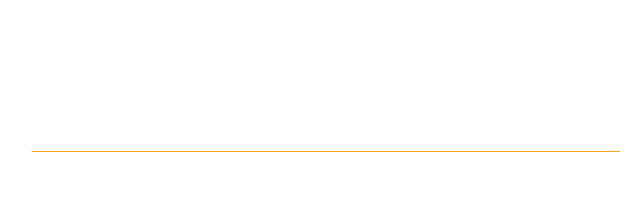
\includegraphics[width=4cm]{figures/1174027/2/soal6.png}
		\centering
		\caption{Hasil SHP Soal 6}
	\end{figure}

	\item Buatlah Script Python dan jelaskan berbaris
	\lstinputlisting[firstline=73, lastline=80]{src/1174027/2/praktikum.py}
	\begin{itemize}
		\item Untuk baris pertama berfungsi untuk memanggil library PYSHP atau shapefile
		\item Untuk baris kedua berfungsi untuk menggunakan atribute Writer yang digunakan untuk membuat file shp,shx, dan dbf. \hfill\break Dengan parameter nama outputnya dan shapeTypenya(shapeType bisa menggunakan angka / namanya).
		\item Untuk baris ketiga digunakan untuk menentukan jenis shapeTypenya.
		\item Untuk baris keempat dan kelima digunakan untuk membuat field yang akan disimpan pada database, dan tipe data yang digunakannya.
		\item Untuk baris keenam digunakan untuk menginputkan data,sesuai dengan jumlah fieldnya.
		\item Untuk baris ketujuh digunakan untuk menginputkan koordinat(x,y), dengan menggunakan line atribute untuk menghasilkan pola line. \hfill\break
		saat menginputkan data, data dengan jumlah koordinat harus sama, karena berkorespondensi 1 - 1.
		\item Untuk Baris kedelapan digunakan untuk mengakhiri proses pembuatan PYSHP.
	\end{itemize}
	\hfill\break
	\begin{figure}[H]
		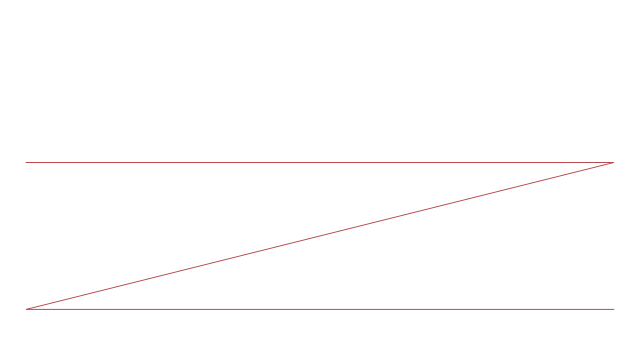
\includegraphics[width=4cm]{figures/1174027/2/soal7.png}
		\centering
		\caption{Hasil SHP Soal 7}
	\end{figure}

	\item Buatlah Script Python dan jelaskan berbaris
	\lstinputlisting[firstline=83, lastline=90]{src/1174027/2/praktikum.py}
	\begin{itemize}
		\item Untuk baris pertama berfungsi untuk memanggil library PYSHP atau shapefile
		\item Untuk baris kedua berfungsi untuk menggunakan atribute Writer yang digunakan untuk membuat file shp,shx, dan dbf. \hfill\break Dengan parameter nama outputnya dan shapeTypenya(shapeType bisa menggunakan angka / namanya).
		\item Untuk baris ketiga digunakan untuk menentukan jenis shapeTypenya.
		\item Untuk baris keempat dan kelima digunakan untuk membuat field yang akan disimpan pada database, dan tipe data yang digunakannya.
		\item Untuk baris keenam digunakan untuk menginputkan data,sesuai dengan jumlah fieldnya.
		\item Untuk baris ketujuh digunakan untuk menginputkan koordinat(x,y), dengan menggunakan polygon atribute untuk menghasilkan pola polygon. \hfill\break
		saat menginputkan data, data dengan jumlah koordinat harus sama, karena berkorespondensi 1 - 1.
		\item Untuk Baris kedelapan digunakan untuk mengakhiri proses pembuatan PYSHP.
	\end{itemize}
	\hfill\break
	\begin{figure}[H]
		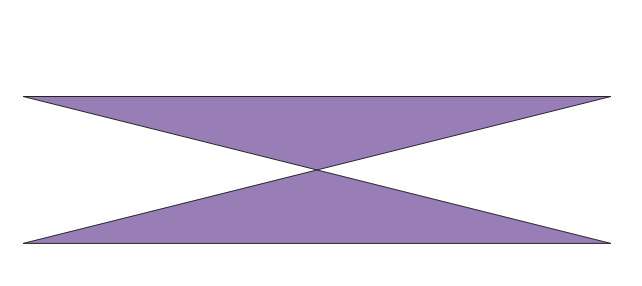
\includegraphics[width=4cm]{figures/1174027/2/soal8.png}
		\centering
		\caption{Hasil SHP Soal 8}
	\end{figure}

	\item Buatlah Script Python dan jelaskan berbaris
	\lstinputlisting[firstline=93, lastline=102]{src/1174027/2/praktikum.py}
	\begin{itemize}
		\item Untuk baris pertama berfungsi untuk memanggil library PYSHP atau shapefile
		\item Untuk baris kedua berfungsi untuk menggunakan atribute Writer yang digunakan untuk membuat file shp,shx, dan dbf. \hfill\break Dengan parameter nama outputnya dan shapeTypenya(shapeType bisa menggunakan angka / namanya).
		\item Untuk baris ketiga digunakan untuk menentukan jenis shapeTypenya.
		\item Untuk baris keempat dan kelima digunakan untuk membuat field yang akan disimpan pada database, dan tipe data yang digunakannya.
		\item Untuk baris keenam dan ketujuh digunakan untuk menginputkan data,sesuai dengan jumlah fieldnya.
		\item Untuk baris kedelapan dan kesembilan digunakan untuk menginputkan koordinat(x,y), dengan menggunakan polygon atribute untuk menghasilkan pola polygon. \hfill\break
		saat menginputkan data, data dengan jumlah koordinat harus sama, karena berkorespondensi 1 - 1.
		\item Untuk Baris kesepuluh digunakan untuk mengakhiri proses pembuatan PYSHP.
	\end{itemize}
	\hfill\break
	\begin{figure}[H]
		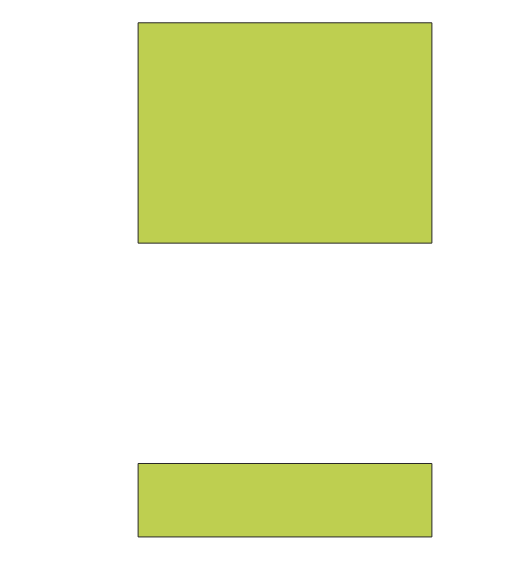
\includegraphics[width=4cm]{figures/1174027/2/soal9.png}
		\centering
		\caption{Hasil SHP Soal 9}
	\end{figure}

	\item Sekarang coba gambar berdasarkan NPM mod 8
	\lstinputlisting[firstline=106, lastline=121]{src/1174027/2/praktikum.py}
	\begin{itemize}
		\item Untuk baris bertama berfungsi untuk mengetahui sisa bagi dari NPM
		\item Untuk baris kedua berfungsi untuk memanggil library PYSHP atau shapefile
		\item Untuk baris ketiga berfungsi untuk menggunakan atribute Writer yang digunakan untuk membuat file shp,shx, dan dbf. \hfill\break Dengan parameter nama outputnya dan shapeTypenya(shapeType bisa menggunakan angka / namanya).
		\item Untuk baris keempat digunakan untuk menentukan jenis shapeTypenya.
		\item Untuk baris kelima dan keenam digunakan untuk membuat field yang akan disimpan pada database, dan tipe data yang digunakannya.
		\item Untuk baris ketujuh dan kedelapan digunakan untuk menginputkan data,sesuai dengan jumlah fieldnya.
		\item Untuk baris kesembilan dan kesepuluh digunakan untuk menginputkan koordinat(x,y), dengan menggunakan polygon atribute untuk menghasilkan pola polygon. \hfill\break
		saat menginputkan data, data dengan jumlah koordinat harus sama, karena berkorespondensi 1 - 1.
		\item Untuk Baris kesebelas digunakan untuk mengakhiri proses pembuatan PYSHP.
	\end{itemize}
	\hfill\break
	\begin{figure}[H]
		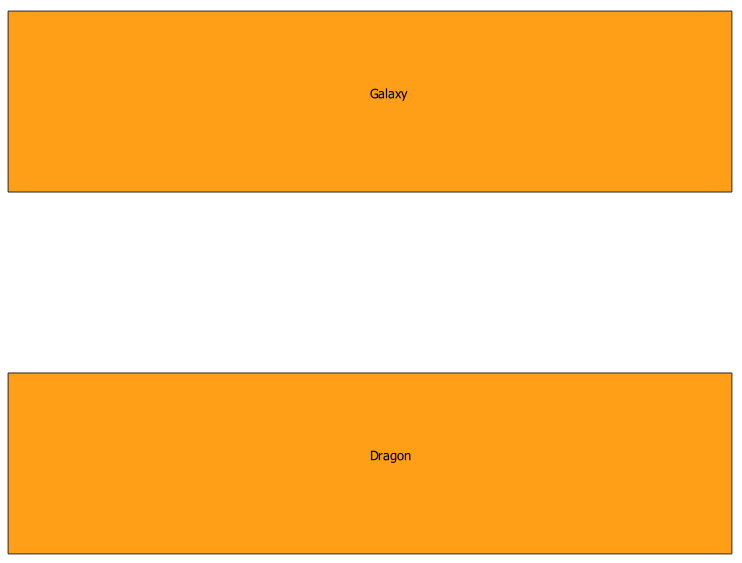
\includegraphics[width=4cm]{figures/1174027/2/soal10.png}
		\centering
		\caption{Hasil SHP Soal 10}
	\end{figure}
\end{enumerate}
\subsection{Link Youtube}
\href{https://youtu.be/Apvppjotft8}{Video Youtube}
\subsection{Plagiarism}
\begin{figure}[H]
	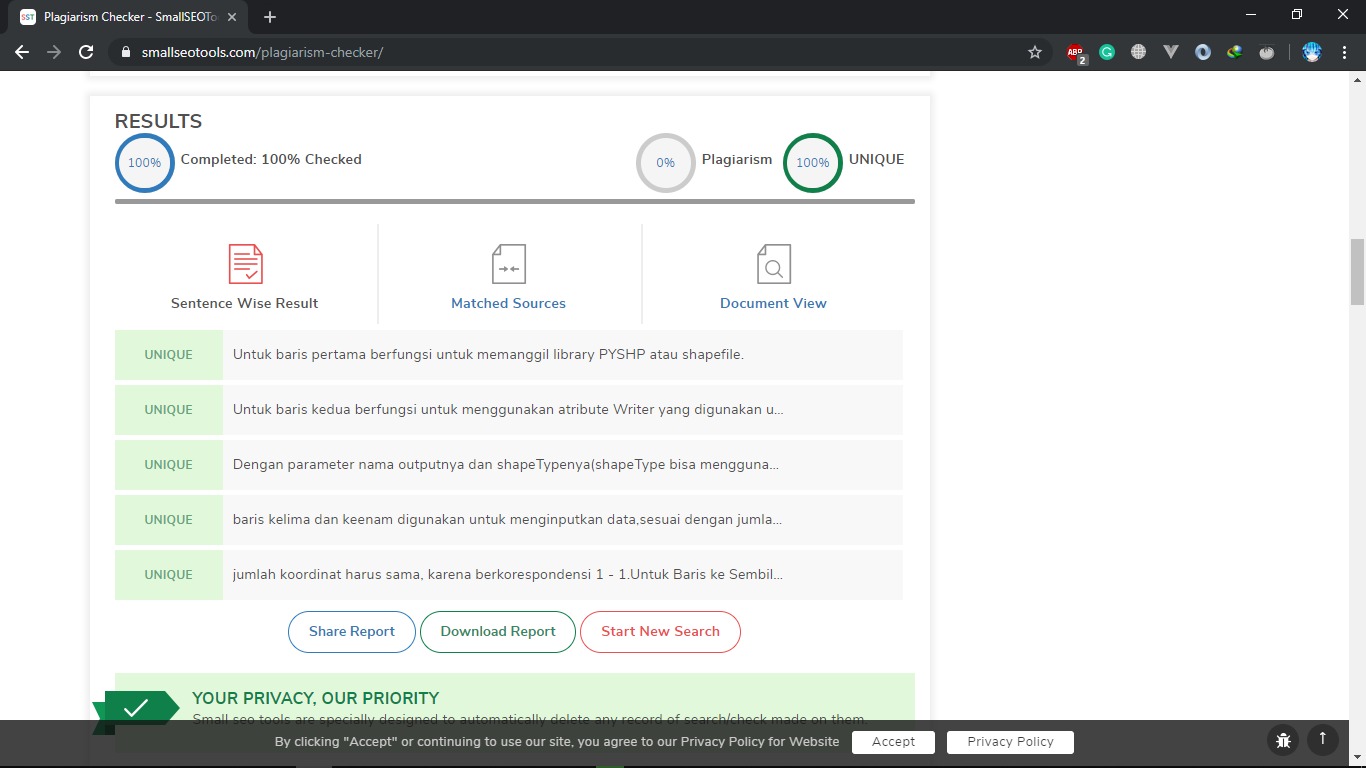
\includegraphics[width=4cm]{figures/1174027/2/bukti_Unique.png}
	\centering
	\caption{Bukti Tidak Melakukan Plagiat}
\end{figure}